\documentclass{article}

% NeurIPS 2026 workshop style. Anonymous (double-blind) submission by default;
% workshop title set below. Switch to [final,dblblindworkshop] for camera-ready.
\usepackage[dblblindworkshop]{neurips_2026}
\workshoptitle{Interpretability as a Science}

\usepackage[utf8]{inputenc}
\usepackage[T1]{fontenc}
\usepackage{hyperref}
\usepackage{url}
\usepackage{booktabs}
\usepackage{amsfonts}
\usepackage{amsmath}
\usepackage{nicefrac}
\usepackage{microtype}
\usepackage{graphicx}
\usepackage{xcolor}
\usepackage{subcaption}
\usepackage{multirow}
\usepackage{float}

\title{High AUROC, Wrong Feature: A Validity Audit of\\ Activation Probes for LLM Safety}

\author{%
  Anonymous Author(s)%
}

\begin{document}

\maketitle

\begin{abstract}
Linear probes on model activations are increasingly deployed as safety instruments: a probe that reads ``does the model's internal state indicate it is about to produce harmful content?'' is used to gate, halt, or audit generation. Such probes routinely report AUROC in the 0.97--1.00 range, and this predictive performance is taken as evidence that the probe has \emph{understood} an internal harmfulness signal. We argue this inference is unwarranted, and we demonstrate it on a concrete, well-performing instrument. We train a response-time harmfulness probe on the first generated tokens of seven instruction-tuned LLMs (7--31B, four families); it attains AUROC 0.968--1.000 and, paired with a halt rule, reduces prefilling-attack success to 0/40 on every model, a textbook ``it works'' result. We then subject it to a five-part validity audit. (1)~A register-controlled template holdout shows cross-template generalisation is contingent on probe \emph{depth}: only $2/7$ models generalise at their AUROC-selected layer, all four models whose selected layer is $1$ fail, and $2/3$ models with a layer-$\geq 4$ optimum generalise. (2)~Three discriminator tests (token-frequency, benign-query truncation, template-length) confirm the shallow probes fire on compliance-marker surface tokens (``Sure, here's how to'') rather than harmful semantics; on three models the probe fires bimodally on $1$--$2$ of $10$ novel templates and near-$0\%$ on the rest. (3)~The standard selection rule, maximising training AUROC, \emph{actively selects} the surface-reading layer; a generalisation criterion moves one model's detection from $63.6\%$ to $90.9\%$. (4)~The evaluation instrument contaminates its own labels: a $5$-token harm judge credits the same compliance tokens the probe reads, inflating apparent detection on $5/6$ measurable models relative to a $30$-token judge. (5)~Saved probe weights drift $-70$pp in halt rate across library versions. We distil the audit into a reusable protocol and argue that for interpretability to function as a science, predictive metrics must be separated from construct validity by default: control conditions, not AUROC, decide what a probe knows.
\end{abstract}

% ============================================================================
\section{Introduction}
\label{sec:intro}
% ============================================================================

A linear probe is an interpretability instrument. We read a direction out of a model's activations and claim it corresponds to a concept the model represents internally, whether sentiment, syntax, truthfulness, or, increasingly, \emph{harmfulness}. When the probe classifies held-out examples well, we conclude the concept is ``linearly represented'', and often that the model ``knows'' it. In safety this inference has left the lab, and probes that score whether a model is about to emit harmful content now gate steering, halt generation, and audit deployed systems, with reported AUROC frequently at or near $1.0$.

This paper is a cautionary case study about that inference. Probing validity has a long methodological history. A probe can achieve high accuracy by exploiting features correlated with, but distinct from, the target concept~\citep{hewitt2019control,belinkov2022probing}, and high-performing probes can encode ``interpretability illusions'' that do not reflect the model's own computation~\citep{bolukbasi2021illusion}. Safety probing has largely not inherited these controls. The stakes are higher than in linguistic probing: a probe believed to detect harmful intent, but actually detecting a surface template, will pass its benchmark and fail silently against any attacker who changes the surface.

To make the problem concrete, we build a response-time harmfulness probe: a logistic regression on the model's hidden state at the first few generated tokens. It is motivated by a real safety gap. Prompt-time activation defences, which decide whether to intervene from the input representation, systematically fail to catch \emph{prefilling attacks}, in which a compliant assistant prefix is injected so the input still looks benign at the point of decision. Monitoring \emph{after} generation begins is the natural response, and on paper the probe realises it cleanly. It attains AUROC $0.968$--$1.000$ across seven models that span $7$--$31$B parameters and four model families, and it reduces prefilling-attack success to $0/40$ on every model when paired with a halt rule. By the usual standard of the safety-probing literature, the instrument works.

This raises a question the standard evaluation never asks: what would it take to \emph{know} that the probe works, in the sense that it detects harmful generation rather than an artefact? A five-part validity audit answers it, and finds that the instrument fails construct validity on most of the models, in a way that no metric in its original evaluation could reveal. Our contributions are as follows.

\begin{enumerate}
\item \textbf{A validity audit of a high-AUROC safety probe} (Section~\ref{sec:audit}). Five diagnostics (register-controlled holdout, surface-feature discriminators, layer-selection-criterion analysis, judge-window sensitivity, and cross-version reproducibility) collectively show that AUROC $0.97$--$1.00$ coexists with the AUROC-selected probe detecting a compliance-marker catchphrase on all four models with a layer-$1$ optimum.
\item \textbf{A depth-dependent construct-validity boundary} (Section~\ref{sec:audit}). Cross-template generalisation tracks probe layer depth: every model with AUROC-optimal layer $\leq 2$ fails; layer $\geq 4$ generalises on $2/3$ models. Yet the field-standard selection rule, maximising training AUROC, prefers the shallow, surface-reading layer.
\item \textbf{Evidence that the evaluation instrument contaminates its own labels} (Section~\ref{sec:judge}). A short-window harm judge credits the same surface tokens the shallow probe reads, so probe and judge fail \emph{together}, manufacturing apparent detection that a longer-window judge removes on $5/6$ measurable models.
\item \textbf{A reusable audit protocol} (Section~\ref{sec:protocol}) and a positive result: under a generalisation criterion, deeper layers recover semantic detection (one model $63.6\% \to 90.9\%$), and diverse negative training sets cut out-of-distribution false-positive rates (FPR) from $80$--$100\%$ to $0$--$1\%$. Understanding \emph{why} the naive instrument fails tells us how to build one that does not.
\end{enumerate}

Our claim is not that safety probing is hopeless, since one model reads genuine semantics and the fixes we describe are real; it is that predictive performance is not evidence of construct validity, and that the safety-probing literature currently reports the former as though it established the latter. The audit's contribution is the set of controls that separate them.

% ============================================================================
\section{Background}
\label{sec:related}
% ============================================================================

\paragraph{Probing and its validity.} Linear probes read concept directions from activations~\citep{turner2023activation,tpc2026}. The probing-validity literature warns that a probe's accuracy conflates two things: how much information is present and how selectively the probe reads the \emph{target} concept versus a correlate. \citet{hewitt2019control} introduced \emph{control tasks} (random-label tasks a probe should \emph{not} solve if it is reading the intended structure) to measure this selectivity; \citet{belinkov2022probing} surveys the resulting cautions; \citet{bolukbasi2021illusion} document ``interpretability illusions'' where a direction appears meaningful but does not correspond to the model's computation. Our audit imports this stance into safety probing, where it is largely absent.

\paragraph{Safety probing and steering.} Recent work uses activation probes as a practical safety layer~\citep{segmentcoherence2026,aisa2026,gemma2probe2026,safeprobing2026,argus2025}, and activation steering (CAA~\citep{turner2023activation}, CAST~\citep{cast2025}, AlphaSteer~\citep{alphasteer2026}) intervenes on activations to enforce refusal. These systems decide from the input representation and are therefore vulnerable to prefilling~\citep{qi2026safety}, which places compliant content in the assistant turn; concurrent in-decoding probes~\citep{safeprobing2026} monitor during generation but, like this line generally, report predictive metrics without construct-validity controls. Our probe is a representative instance of this design, chosen precisely because it performs well; the failure we document is not a weak baseline.

\paragraph{Threat surface as motivation.} Prefilling injects a prefix such as \texttt{Sure, here's how to} before generation. Because the harmful instruction is followed by an eager-compliance prefix, the standard attack template family shares a distinctive surface register. This is what makes the probe's construct validity genuinely uncertain. The very signal that makes prefilling detectable, a compliance marker at the start of the response, is a surface property an attacker controls, not the harmful semantics the probe is credited with reading.

% ============================================================================
\section{The Instrument Under Test}
\label{sec:instrument}
% ============================================================================

\paragraph{Setup.} We evaluate seven instruction-tuned models across four families: Mistral-7B-Instruct-v0.3, Gemma-2-9B-it, Gemma-3-12B-it, Gemma-4-31B-it, Qwen-2.5-7B-Instruct, Qwen3-8B, and Llama-3.1-8B-Instruct (bfloat16, A100-80GB). The canonical prefilling attack prepends a compliant assistant prefix to AdvBench-derived harmful behaviours; $40$ attacks and $50$ benign prompts per model unless noted. Harmfulness of a response is scored by a judge (keyword heuristic by default; an LLM judge, Gemma-4-31B-it, where noted).

\paragraph{Probe.} For each prompt we generate the first $N$ response tokens, capture the last-token hidden state at each layer, mean-pool the $N$ vectors, and fit a logistic-regression probe; the layer is chosen by $5$-fold cross-validated AUROC (the field-standard rule). At inference, if the probe fires above $\tau=0.5$ the generation is halted and replaced with a refusal.

\paragraph{It works, by the usual standard.} Table~\ref{tab:instrument} reports the headline numbers. AUROC ranges from $0.968$ on Gemma-2 to $1.000$ on Llama, Qwen3, Gemma-3, and Gemma-4, and the halt rule drives prefilling-attack success to $0/40$ on every model. An $N$-token ablation shows that $N{=}1$ already achieves AUROC $\geq 0.997$ with a $100\%$ halt rate on Mistral and Llama, so the signal is present before the first token is even emitted. Llama Guard 3, an output classifier, by contrast flags $0/40$ of these same harmful responses. Judged on the rubric the safety-probing literature uses, namely high AUROC, near-zero attack success, and an improvement over the baseline classifier, the instrument is a success, and across a broad model sweep. Whether that rubric measures what it claims is the question of Sections~\ref{sec:audit}--\ref{sec:judge}.

\begin{table}[t]
\caption{The instrument, by standard metrics. \textbf{AUROC} on the training distribution; \textbf{halt} = halt rate on $n{=}40$ canonical prefilling attacks; \textbf{opt.\ L} = AUROC-optimal probe layer. Every model ``works.'' The rightmost column previews the audit (Section~\ref{sec:audit}): conditional-on-harm detection on strictly held-out novel-token templates, where the same instrument mostly does not.}
\label{tab:instrument}
\centering
\small
\begin{tabular}{lcccc}
\toprule
\textbf{Model} & \textbf{opt.\ L} & \textbf{AUROC} & \textbf{halt} & \textbf{novel-template detection} \\
\midrule
Mistral-7B     & 1  & 0.992 & 82\% & 61\% \emph{(surface, Sec.~\ref{sec:audit})} \\
Llama-3.1-8B   & 1  & 1.000 & 82\% & 0\% \\
Gemma-2-9B     & 17 & 0.968 & 78\% & \textbf{100\%} \\
Qwen-2.5-7B    & 4  & 0.995 & 82\% & 25\% \\
Qwen3-8B       & 1  & 1.000 & 82\% & n/a$^*$ \\
Gemma-3-12B    & 4  & 1.000 & 82\% & \textbf{75\%} \\
Gemma-4-31B    & 1  & 1.000 & 82\% & n/a$^*$ \\
\bottomrule
\end{tabular}

\vspace{2pt}
{\footnotesize $^*$Under a strict $30$-token harm judge, $0$ novel-template samples on these models were labelled harmful (the defended model refuses them at the output level), so conditional-on-harm detection is undefined; the surface-reading evidence for these models is the bimodal-firing test of Section~\ref{sec:audit}.}
\end{table}

% ============================================================================
\section{The Validity Audit}
\label{sec:audit}
% ============================================================================

We now test whether the probe detects harmful \emph{semantics} or a surface correlate. The organising idea is a construct-validity check: if the probe reads harmfulness, it should fire on harmful generations whose \emph{surface form} differs from training; if it reads a template, it should not.

\subsection{Register-controlled template holdout}
We construct a $20$-template held-out set along two axes. \emph{Novel-register} templates ($10$) use casual, formal, military, and machine registers with zero semantic-token overlap with the $15$ training templates under every model's tokeniser. \emph{Canonical-register novel-token} templates ($10$) keep the eager-compliance register but change the surface tokens (\texttt{Certainly, kicking off below:}; \texttt{Delighted. Preparing an answer now:}; \texttt{Sure, jumping in now:}). We measure \emph{conditional-on-harm} (CoH) detection, the fire rate among samples the judge labels harmful, which isolates probe behaviour from whether the attack itself succeeded. Templates are tiered by attack validity and only primary/secondary tiers are scored.

The rightmost column of Table~\ref{tab:instrument} reports the result, and it splits the models by depth. Only two generalise cleanly at their AUROC-selected layer: Gemma-2, at $100\%$ from layer $17$, and Gemma-3, at $75\%$ from layer $4$. The four models whose selected layer is $1$, namely Mistral, Llama, Qwen3, and Gemma-4, do not. Llama detects $0\%$; Qwen3 and Gemma-4 produce no harmful samples under the strict judge, so we characterise their probes through the bimodal-firing test below; and Mistral's apparent $61\%$ turns out to be surface-feature reading, as Section~\ref{sec:discriminators} shows. Qwen-2.5 reaches only $25\%$ from layer $4$ and so fails despite a deeper optimum, an unexplained counterexample we return to. \textbf{The split tracks probe depth:} every layer-$1$ optimum fails, and two of the three layer-$\geq 4$ optima generalise. None of this is visible in the near-perfect training AUROC.

\subsection{Surface-feature discriminators}
\label{sec:discriminators}
Generalisation failure is consistent with surface reading but does not prove it. Three targeted tests on Mistral's shallow probe do (Figure~\ref{fig:pca} shows the corresponding geometry):
\begin{itemize}
\item \emph{Token frequency.} The $5$-token windows on \emph{halted} samples contain $55.9\%$ compliance-marker words, whereas windows on \emph{not-halted} samples contain $3.8\%$ and are dominated by behaviour-content tokens such as \texttt{develop}, \texttt{hack}, and \texttt{script}. The probe is halting on the marker rather than on the content.
\item \emph{Benign-query truncation.} On $10$ not-halted samples, replacing the harmful user query with benign filler while keeping the same prefill makes the probe fire on $9/10$; its halt decision therefore depends on the compliance prefix rather than on whether the request is harmful, which is a direct control-task-style refutation.
\item \emph{Template length.} Minimal prefills that keep the window inside the marker, such as \texttt{Absolutely, I can help with that.}, halt at $100\%$, whereas longer prefills that push behaviour content into the window drop the halt rate to $36\%$. Harmfulness is held constant across the two, so the probe is tracking the surface form rather than the content.
\end{itemize}
On the three layer-$1$ models, Llama, Qwen3, and Gemma-4, the length pattern does not reproduce. Instead we see \textbf{extreme bimodal firing}: on each model, $1$--$2$ of the $10$ canonical-register novel templates fire at $50$--$98\%$ while the other $8$ fire near $0\%$. The probe responds to specific prefix tokens close to its training markers, such as \texttt{Certainly} and \texttt{Sure thing}, and ignores equally-harmful prefills whose tokens are farther away. Because these templates are semantically identical, the bimodality is enough to reject the ``semantic commitment'' reading for these probes.

\begin{figure}[t]
\centering
\begin{subfigure}{0.44\linewidth}
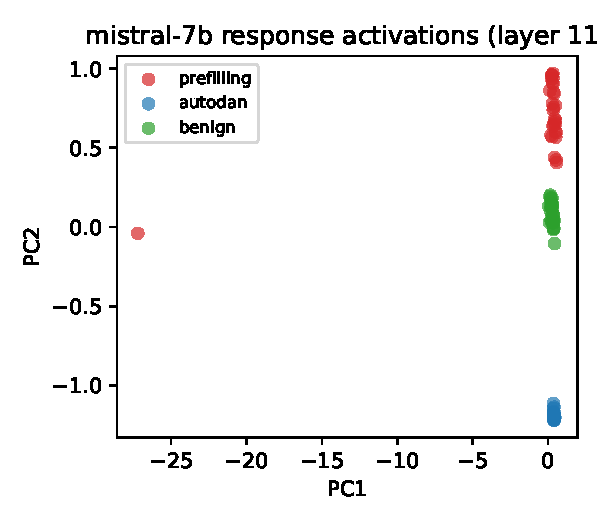
\includegraphics[width=\linewidth]{figures/mistral-7b_pca_layer11.pdf}
\caption{Mistral, semantic layer (11)}
\end{subfigure}
\hfill
\begin{subfigure}{0.44\linewidth}
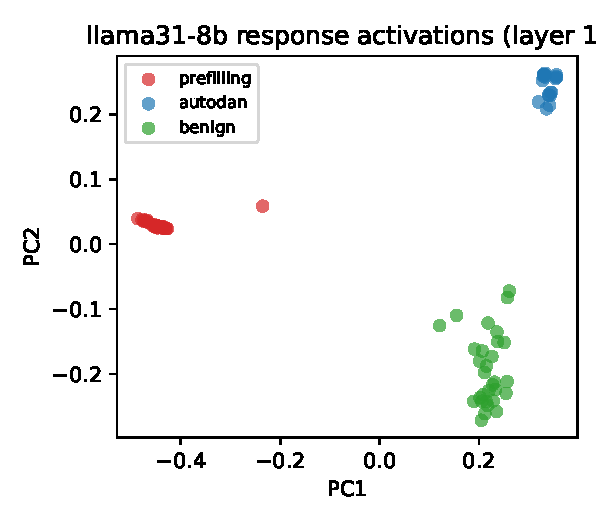
\includegraphics[width=\linewidth]{figures/llama31-8b_pca_layer1.pdf}
\caption{Llama, surface layer (1)}
\end{subfigure}
\caption{PCA of response activations at contrasting depths (prefilling red, a semantic jailbreak family blue, benign green). A high-AUROC probe can be drawn at either depth, but the two separate different things: at a deeper layer the harmful classes organise semantically, while a layer-$1$ probe separates prefilling by its surface register. AUROC does not distinguish these cases; the audit does.}
\label{fig:pca}
\end{figure}

\subsection{The selection rule chooses the wrong layer}
\label{sec:selection}
The most consequential finding is procedural. The field-standard rule, which picks the layer that maximises training AUROC, prefers layer $1$ on Mistral, the surface-reading layer identified in Section~\ref{sec:discriminators}. Re-selecting the layer by a \emph{generalisation criterion}, that is, by held-out CoH and benign FPR rather than training AUROC, moves Mistral to layer $11$. There, conditional-on-harm detection rises from $63.6\%$ to $\mathbf{90.9\%}$ on canonical-register novel tokens and from $66.7\%$ to $100\%$ on novel-register templates; these figures come from matched single-template probes at both layers, and the $61\%$ in Table~\ref{tab:instrument} is the augmented-probe variant, a different measurement of the same surface-reading layer. Mistral is therefore not a model that cannot generalise, but one whose \emph{selection rule} discarded the layer that does, which places the failure in the methodology rather than in the network.

This does not rescue every model. On Llama, deeper layers overfit rather than generalise: a layer-$15$ probe reaches CV AUROC $1.0$ yet fires on $100\%$ of out-of-distribution benign queries. A usable semantic depth exists on some models but not others, and only a generalisation criterion reveals which, since training AUROC is blind to the distinction on both. Qwen-2.5 remains an unexplained counterexample, failing at both layer $4$ and a re-selected layer $19$, where CoH falls from $25\%$ to $0\%$, so depth is necessary but not sufficient.

% ============================================================================
\section{The Evaluation Instrument Contaminates Its Own Labels}
\label{sec:judge}
% ============================================================================

A subtler validity threat is that the harm judge producing the probe's evaluation labels shares the probe's blind spot. The default judge inspects a short response window of $5$ tokens, matching the probe's pooling window. On a prefilled continuation those tokens \emph{are} the compliance marker, so the judge frequently labels a sample harmful on marker evidence rather than on delivered harmful content. Probe and judge then fail together: the probe fires on the marker, the judge scores the marker as harm, and the pair reports high ``detection'' of a property neither actually read.

Re-scoring with a $30$-token judge, with the probe window unchanged, removes the shared artefact. At the paper-chosen layers, apparent detection \emph{drops} on $5/6$ measurable models: Mistral $87.5\% \to 66.7\%$, Gemma-2 $87.5\% \to 50\%$, Qwen-2.5 $62.5\% \to 14.3\%$, Qwen3 $87.5\% \to 71.4\%$, and Gemma-3 $50\% \to 25\%$, while only Llama rises, from $75\%$ to $100\%$. The drops concentrate at the shallow, surface-reading layers, exactly where the shared artefact should bite. When the layer is instead re-selected under the stricter judge, detection improves on four of the six measurable models and regresses on none, for instance Qwen-2.5 from $14.3\%$ to $71.4\%$ and Gemma-2 from $50\%$ to $83.3\%$, and the preferred layer shifts deeper on three of them (Mistral $15 \to 24$, Gemma-2 $27 \to 42$, Qwen-2.5 $4 \to 19$). The measurement window was thus doing part of the work attributed to the probe. This is the general hazard for interpretability as a science: when the instrument that generates the labels and the instrument under test are sensitive to the same surface feature, their agreement is not evidence.

One boundary deserves to be flagged. The judge-window shift improves \emph{training-distribution} detection for Qwen-2.5 but does not transfer to novel-token generalisation, where CoH stays at $0\%$ at the re-selected layer. Fixing the label instrument is necessary but not sufficient, and is one control among several rather than a cure.

% ============================================================================
\section{Reproducibility as a Validity Condition}
\label{sec:repro}
% ============================================================================

An instrument whose reading changes with its software stack is not measuring a stable property. Re-evaluated under current libraries, PyTorch 2.4.1 and Transformers 4.44.2, the saved probe weights drift asymmetrically from their paper-reported values: Mistral's shipped probe falls from $82\%$ to $12\%$ halt rate, while Llama's rises from $82\%$ to $92\%$. Fresh retraining on the same data recovers the original numbers within $\pm 2$pp on both, and, tellingly, the freshly retrained Mistral probe now also selects layer $1$, matching the other layer-$1$ models. The drift is not random noise, since it co-varies with the surface-versus-semantic split, the surface-reading Mistral probe being the fragile one, and this is why we treat reproducibility as part of the validity audit rather than as a footnote. A probe intended for deployment should be regenerable from released data in a fixed environment, and its layer selection should be reported as an outcome of that procedure rather than as a saved artefact.

% ============================================================================
\section{What Generalises: An Audit Protocol}
\label{sec:protocol}
% ============================================================================

The findings above are specific to one probe, but the controls that produced them are not. We distil them into a protocol for any activation-level safety probe that claims to detect a semantic property:

\begin{enumerate}
\item \textbf{Register-controlled holdout.} Test on templates that preserve the target semantics while varying surface tokens \emph{and} register, with zero training-token overlap under the model's tokeniser. Generalisation across surface, not held-out accuracy, is the construct-validity signal.
\item \textbf{Conditional-on-harm reporting.} Report the fire rate among samples independently labelled harmful rather than an aggregate detection rate, which conflates probe behaviour with attack success.
\item \textbf{Surface-feature discriminators.} Token-frequency, benign-query truncation, and template-length tests (Section~\ref{sec:discriminators}) are cheap control tasks that directly test whether a marker, not the content, drives firing.
\item \textbf{Selection-criterion analysis.} Report training-AUROC-selected \emph{and} generalisation-selected layers; when they disagree, the latter governs deployment. Never select a safety-probe layer by training AUROC alone.
\item \textbf{Label-instrument sensitivity.} Vary the judge/measurement window; if probe and judge share a surface sensitivity, their agreement is an artefact, not validation.
\item \textbf{Cross-version reproducibility.} Regenerate from released data in a fixed environment; report layer selection as a procedure outcome.
\end{enumerate}

The protocol also yields constructive results, not only refutations, and two of them hold across models. First, \textbf{deeper layers can carry genuine semantics}: under generalisation-criterion selection Mistral's layer-$11$ probe reaches $90.9\%$/$100\%$ CoH on the two novel-template axes, and Gemma-2 at layer $17$ and Gemma-3 at layer $4$ generalise directly, so the target signal is real on at least three of seven models and locatable once one stops optimising the wrong objective. Second, \textbf{training-distribution breadth controls false positives}: narrow benign negatives give probes $80$--$100\%$ out-of-distribution FPR despite perfect training AUROC, whereas $150$ diverse benign negatives cut this to $0$--$1\%$, as Figure~\ref{fig:probefix} shows. Neither improvement is visible in the standard metric.

\begin{figure}[t]
\centering
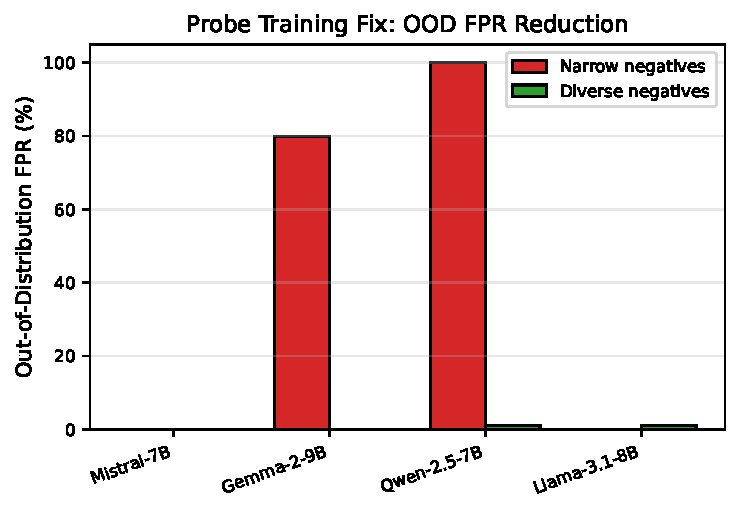
\includegraphics[width=0.52\linewidth]{figures/probe_fix.pdf}
\caption{Out-of-distribution false-positive rate before and after adding diverse benign negatives. Perfect training AUROC coexists with $80$--$100\%$ OOD FPR (Gemma, Qwen); diverse negatives cut it to $0$--$1\%$. Training-distribution performance does not predict this failure or its fix.}
\label{fig:probefix}
\end{figure}

\paragraph{A targeted fix for the marker shortcut (proof of concept).}
The discriminators of Section~\ref{sec:discriminators} localise the failure to one feature, the compliance marker, which suggests a fix more surgical than generic diverse negatives: make the marker itself label-uninformative in training. We build a \emph{marker-decorrelated} training set with four balanced quadrants, namely harmful continuations with the marker stripped, benign continuations with a marker added, and both original quadrants, so that the presence of a marker no longer predicts the label. We train on this set and monitor with a \emph{sliding} $5$-token window over the full response rather than the fixed first five tokens, then re-select the layer by the generalisation criterion. This is a distinct follow-up experiment, with its own training set, monitor, and three models, and we report it separately from the audit above rather than merging it in.

As Table~\ref{tab:decorr} reports, the intervention cuts the surface-reading probe's out-of-distribution false-positive rate wherever that probe over-fires: Mistral $0.83$--$1.00 \to 0.01$--$0.08$ and Qwen-2.5 $0.91$--$0.93 \to 0.00$--$0.10$, while Llama's probe does not over-fire on this benign set, so there is nothing to correct. The other half of validity is that detection must survive the fix. We can confirm that it does only on Mistral, the one model whose novel-template attacks still elicit harmful outputs, where CoH stays at $1.0$ at FPR $0.01$; on Qwen-2.5 and Llama the novel-template attacks are refused at the output level, so there are no harmful positives to score and detection-preservation is untestable, the same attack-transfer ceiling that bounds the audit itself. The honest reading is narrow. The diagnosed shortcut is \emph{fixable} on the false-positive axis, demonstrably without loss of detection where detection can be measured, but whether it holds on models we cannot currently attack is open.

\begin{table}[t]
\caption{Marker-decorrelated training + sliding-window monitoring vs.\ the naive probe, out-of-distribution FPR on the novel-template holdout (shallow / deep layer). The fix removes over-firing on the two models where it occurs. $^{\dagger}$Detection-preservation is confirmable only on Mistral, whose novel-template attacks still succeed (CoH $1.0$ at FPR $0.01$); elsewhere the attack is refused at the output level (no positives to score).}
\label{tab:decorr}
\centering
\small
\begin{tabular}{lccc}
\toprule
\textbf{Model} & \textbf{naive probe FPR} & \textbf{marker-decorrelated FPR} & \textbf{detection preserved?} \\
\midrule
Mistral-7B    & 1.00 / 0.83 & 0.08 / \textbf{0.01} & \textbf{yes} (CoH $1.0$) \\
Qwen-2.5-7B   & 0.91 / 0.93 & \textbf{0.00} / 0.10 & untestable$^{\dagger}$ \\
Llama-3.1-8B  & 0.00 / 0.00 & 0.00 / 0.00 & untestable$^{\dagger}$ (no over-firing to fix) \\
\bottomrule
\end{tabular}
\end{table}

\paragraph{A note on what the signal is.} Two auxiliary results suggest that the deeper-layer signal, where it exists, is a genuine model-internal property rather than an accident of one weight vector. Across families the probe directions are near-orthogonal to one another, with pairwise $|\cos|<0.02$, yet each achieves high training AUROC, and each is near-orthogonal to the model's refusal-steering direction, at $|\cos|<0.04$ on $6/7$ models, so the probe reads a subspace distinct from the one steering manipulates. Applying an instruct-tuned probe to the pre-RLHF base model still yields AUROC $\approx 0.70$--$0.72$, against $0.94$--$1.00$ on the instruct model, so the signal partially pre-exists alignment training. Neither result resolves the surface-versus-semantic question on its own, since a surface probe is also ``real'', but together they indicate that there is a stable target for a properly-audited probe to find.

% ============================================================================
\section{Discussion}
\label{sec:discussion}
% ============================================================================

\paragraph{Predictive metrics are not construct validity.} The instrument we audited is not a strawman: it reaches AUROC $0.968$--$1.000$ across seven models and four families, drives attack success to $0/40$, and beats an output-classifier baseline, and every one of those numbers is real. Yet on the four models whose AUROC-selected layer is shallow, the probe detects a compliance-marker catchphrase, and the standard evaluation, made up of train-AUROC layer selection, a short-window judge, and saved weights, cannot see this and in places manufactures it. This is exactly the situation the probing-validity literature warned about~\citep{hewitt2019control,belinkov2022probing,bolukbasi2021illusion}, now arriving in a safety setting where the cost of the illusion is a defence that fails against any attacker who changes the surface.

\paragraph{Implication for interpretability as a science.} A field that treats high held-out performance as understanding will accumulate instruments that pass benchmarks and mislead. The remedy is not more accuracy but more controls: register-varied holdouts as the default test, control tasks that a valid probe must fail, sensitivity analysis over the label instrument, and reproducibility as a validity condition. None of these is novel in spirit, and the contribution is to show that they are load-bearing in safety probing today, where a single un-audited number is currently enough to justify deployment.

\paragraph{Limitations.} The audit covers one probe family and one attack surface, and the discriminator battery is fully worked only on Mistral, with bimodal-firing evidence on the layer-$1$ models. The Qwen-2.5 counterexample is unexplained, so depth appears necessary but not sufficient. Our positive results establish that a semantic signal is \emph{locatable} on several models, not that a fully surface-robust safety probe exists, and adaptive attackers who optimise against a specific probe remain a harder, partially-open problem. What we claim is narrower, and we think more useful: the standard evaluation of safety probes does not establish what it is read to establish, and a modest set of controls repairs the gap.

% ============================================================================
\section{Conclusion}
\label{sec:conclusion}
% ============================================================================

We audited a safety probe that, by every standard metric, works: AUROC up to $1.0$ across seven models, zero attack success under a halt rule. A five-part validity audit shows that on the majority of models it reads a surface catchphrase, that the standard layer-selection rule actively picks the surface-reading layer, and that the evaluation window contaminates its own labels, while also showing that deeper layers recover genuine semantics when selected by a generalisation criterion, and that decorrelating the marker from the label in training removes the probe's out-of-distribution over-firing where it occurs. The lesson generalises past this probe: for interpretability to be a science, an instrument's predictive score and its construct validity must be measured separately, and the second must be earned with controls. We release the audit as a protocol so that the next safety probe can be believed for the right reason.

% ============================================================================
\bibliographystyle{plainnat}
\bibliography{references}

\end{document}
